\begin{itemize}
\item General circuit (right now a highpass)
\item Plotting (linear -> semilog -> loglog)
\item RC and RL circuits (analysis and design)
\begin{itemize}
\item Highpass filter
\item Lowpass filter
\end{itemize}
\item RLC circuits (analysis and design)
\begin{itemize}
\item Bandpass
\item Bandstop/notch
\item Second-order Highpass
\item Second-order Lowpass
\end{itemize}
\item RCRC circuits (Commentary on ease of construction)
\end{itemize}


When we talk about analyzing filters, what we mean is how does the output voltage respond to different frequencies.  We call this the {\bf freqeuncy response} of the circuit.  In practice, this results in solving for the output voltage while keeping $\omega$ a variable.  Figure \ref{fig:CircuitRC} shows an AC source connected to a capacitor and resistor in series.

\begin{figure}
   \centering
%  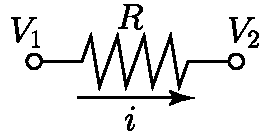
\includegraphics[width=0.5\linewidth]{figures/ohmsLaw}
  
\includegraphics{figures/toDo}
  \caption{A simple circuit composed of a source and two components.}
  \label{fig:CircuitRC}
\end{figure}

Our goal here is to find the frequency response of the output voltage.  We know that $Z_C=\frac{1}{j\omega C}$ and $Z_R = R$.  From voltage division, we obtain the following:
\begin{equation} \label{eq:CircuitLC}
  V_{out} = V_s \frac{R}{R + \frac{1}{j \omega C}}
\end{equation}

Simplified, we can rewrite this as:
\begin{equation}
  \frac{V_{out}}{V_s}=\frac{j \omega RC}{1 + j\omega RC}
\end{equation}

At this point, we either feed this into a program, which can calculate the response over a wide variety of $\omega$ values, or we look into some limits. Specifically, we'd like to find the limit as $\omega$ approaches zero and infinity.

\begin{align}
  \lim_{\omega \to 0} \frac{j \omega RC}{1 + j\omega RC} &= \frac{j (0) RC}{1 + j (0) RC} = 0 \\
  \lim_{\omega \to \infty} \frac{j \omega RC}{1 + j\omega RC} &= \frac{j RC}{j RC} = 1
\end{align}

If we want to plot the response by hand, we need to look at one more value, typically called the {\bf breakpoint frequency}, $\omega_b$.  This is defined as the freqency at which the magnitude of impedance of the two components are equal ($|Z_R| = |Z_C|$):
\begin{align*}
  \left|\frac{1}{j\omega_b C}\right| &= R &
  \frac{1}{\omega_b C} &= R &
  \omega_b &= \frac{1}{RC}
\end{align*}
  
If we plug this back into our frequency response, we find the following:
\begin{align*}
  \frac{V_{out}}{V_s}&=\frac{j RC\left(\frac{1}{RC}\right)}{1 + j RC \left(\frac{1}{RC}\right)} \\
  \frac{V_{out}}{V_s}&=\frac{j}{1+j} \\
  \left|\frac{V_{out}}{V_s}\right|&=\frac{|j|}{|1+j|}=\frac{1}{\sqrt{2}}
\end{align*}

In fact, this is an equivalent definition of the breakpoint frequency.  Our breakpoint occurs when the magnitude of our frequency response is exactly $\sqrt{2}$.

Let's do the other option.  If we have access to a computer, we can plot the amplitude and phase angle of the frequency response as seen in Figure \ref{fig:freqResponseLinear}.  This plot is useful, but we can change our axes to see things a little cleaner.

\begin{figure}
   \centering
%  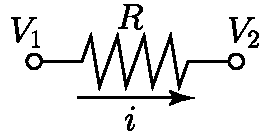
\includegraphics[width=0.5\linewidth]{figures/ohmsLaw}
  
\includegraphics{figures/toDo}
  \caption{The frequency response of the circuit using linear axes.}
  \label{fig:freqResponseLinear}
\end{figure}

Figure \ref{fig:freqResponseLog} shows a log-log plot of the frequency response. In this plot, $\omega$ is replaced in the $x$-axis by $\log(\omega)$ and $\left|\frac{V_{out}}{V_s}\right|$ is replaced by $\log\left(\left|\frac{V_{out}}{V_s}\right|\right)$.  Doing so, the behaviour of the circuit stands out very clearly.  Note that the phase angle $\phi$ did not change between Figures \ref{fig:freqResponseLinear} and \label{fig:freqResponseLog}.

\begin{figure}
   \centering
%  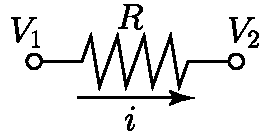
\includegraphics[width=0.5\linewidth]{figures/ohmsLaw}
  
\includegraphics{figures/toDo}
  \caption{The frequency response of the circuit using logarithmic axes.}
  \label{fig:freqResponseLog}
\end{figure}

So what's happening?  Starting at high frequencies, the response is fairly constant until you hit the break point, and then it drops off logarithmically as you decrease the frequency.  To describe this, we say that we allow high frequencies to {\it pass through}.  In shorter terms, this is a {\bf highpass filter}.
